% !TeX root = ../thesis.tex
%*****************************************************************************************
%*********************************** Second Chapter ***************************************
%*****************************************************************************************



\label{ch:Chap2}
\chapter{Jets and Macrospicules}

%%%%%%%%%%%%%%%%%%%%%%%%%%%%%%%%%%%%%%%%%%%%%%%%%%%%%%%%%%% PAPER TEXT %%%%%%%%%%%%%%%%%%%%%%%%%%%%%%%%%%%%%%%%%%%%%%%%%%%%%%%%%%%%%%%%%%%%%%%%%%%%%%


The appearance of thin, explosive features with a relatively short lifespan has for a long time, been a part of solar physics.
Spicules were first observed in 1877 by a Vatican observer, Angelo Secchi.
This was aided by their sheer ubiquity, they were distinctly visible at the solar limb nearly all the time.
However the larger-scale, more infrequent jets were more difficult to observe, particularly with early techniques.

\section{The ejecta zoo}


\subsection{Spicules}
Jets and jet-like features are observed throughout the solar atmosphere, and as such a review of the topic is in order.
As has already been discussed, spicules are among the smallest jets formed in the solar atmosphere. 
Most easily observed at the limb, they are long thin structures appearing brightly at the solar limb \cite{Beckers1972}.
Spicules are found in the chromosphere, regularly observed in the H$\alpha$, He II $30.4$ nm, Ca II and Si IV.
Work by \cite{DePontieu2007} divided spicules into two populations, Type-1 and Type-2, with Type-1 being long lived while Type-2 have distinctly shorter lifetimes but are significantly more explosive and grow to much longer lengths.
Type-1 spicules have an uprising speed of approximately $20$ km s$^{-1}$ and extend to $1$ Mm in height with lifetimes of $10$ mins, whereas the Type-2 spicules have been shown to extend approximately $5$ Mm into the atmosphere and last for an average of $1$-$2$ mins. 
The most comprehensive difference between the two is in the overall evolution of the feature.
Type-1 spicules are observed to have a parabolic evolution, \emph{i.e.} their tip traces out a ballistic arc when plotted against time.
Conversely, Type-2 spicules are observed to dissipate or vanish as they evolve, and are primarily observed in the quiet Sun and coronal holes.
Type-1 develop in active regions, and as such Type-2 are far more numerous when recorded in a study such as \cite{Pereira2012}.

\begin{figure}
	\centering
	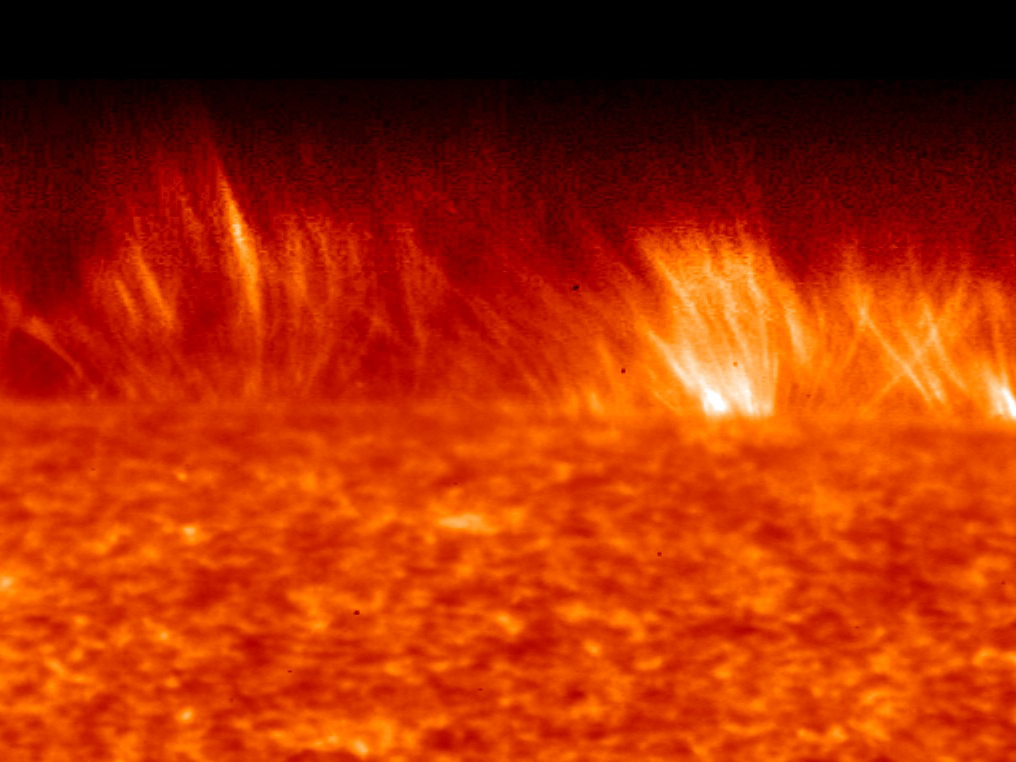
\includegraphics[scale=0.4]{Chapter2/Figs/spicules_at_limb}
	\caption{Spicules as observed by at the solar limb using the new IRIS instrument observing at transition region temperatures.
		\url{http://www.nasa.gov/sites/default/files/images/751917main_highres4_full.jpg}}
\end{figure}

Spicules are visible on the disk as well, but here they are seen as dark thin structures against the bright lower chromosphere.
These were initially named mottles and fibrils, but have since been inherently linked with spicules - see \cite{DePointeu2007MF}.

Since these initial propositions, however, there has been doubt cast as to whether this is the case or not. 
\cite{Zhang2012} found no statistical separation of populations within spicules.
However, \cite{Pereira2014} have presented evidence that Type-2 spicules disappear from Ca II and reappear in the hotter Si IV and Mg II lines. .
This would imply that spicules are heating as they accelerate through the atmosphere.
Whether this is because the underlying formation mechanism is different or because there is sufficient energy in the creation of the spicules to cause heating as they propagate through the atmosphere, has yet to be made clear. % perhaps something like 'creation' might be a better word than 'initialisation' here. They're not Python objects :P

The formation of spicules is still a matter of much debate given our currently limited ability to examine small scales in current observations. 
However, when observations are unable to provide explicit results, numerical and analytic approaches are utilised to fill in the gaps.
\cite{DePointeu2004} outline a mechanism for the formation of spicules which originates in the photosphere based on an anaytic model.
\emph{P}-mode oscillations cannot pass through the photosphere due to the minima in the global temperature.
However, leakage can occur in specific circumstances, allowing energy to transfer through this gap, until temperatures become high enough to allow propagation to start again.
Essential to this model is the inclination of the background magnetic field.
The authors report that an inclined field vastly increases the cut-off frequency of waves tunnelling through the atmosphere. 
The lower density in the upper solar atmosphere causes the photospheric velocity generated by the \emph{p}-modes to steepen into shocks, which leave an oscillating wake in the chromosphere, the spicule.

However this is only one of many competing theories.
\cite{Takeuchi2001} demonstrate a magnetic reconnection model driving formation of spicules, whereas \cite{Martinez2011} formed a $3$ dimensional model utilising the Lorentz force to push plasma across the solar surface until it meets vertical magnetic field which forces the plasma upwards.
\cite{Hollweg1982} demonstrate that a quasi-impulsive source in the photosphere is capable of generating a chain of rebound shocks in the chromosphere, causing the formation of a spicule.

A particularly pertinent model is proposed by \cite{Moore2011spic_recon}, in which magnetic reconnection is instigated by granule-sized 'magnetic bubbles'.
This is applicable, as spicules are generally observed to form on the intergranular lanes.
The authors propose that Type-2 spicules are an analogue for X-ray jets (more on which later).
In this scenario, magnetic bipoles emerge from the photosphere which then interacts with the ambient field of the lower chromosphere, forming a raft of reconnection external to the bipole.
During this reconnection, the interior of the bipole remains inert, while the outermost sections of the structure are released causing a 'sling shot snapping' of the magnetic reconnected field lines producing an upward jet (Type-2 spicule), Alfven waves propagating up the ambient magnetic field lines and a fast MHD wave upwards across the magntic field.

The advantages of this scenario for reconnection are that the environment which generates these spicules is extremely common in the solar atmosphere.
The scenario here is particularly convenient as it also answers questions with respect to heating of the solar atmosphere.
As a result of reconnection between the canopy region which forms over the granules and the more open magnetic fields higher in the atmosphere, shocks and waves are formed, which propagate upwards.
The dissipation of the energy within these disturbances has been proposed on numerous occasions to be the central source of heating of the corona \cite{Klimchuck2012, Kudoh1999, Athay2000}. 

What becomes evident, after all of these models are formed, is that none of them generate both Type-1, and Type-2 spicules.
It is therefore likely that they are indeed two separate features.

\subsection{X-ray Jets}
Throughout the solar atmosphere, we observe much larger jet-like features than spicules.
They have been observed extensively, and not solely in the chromosphere.
The first observations of more large scale jets were undertaken using the Soft X-Ray telescope on board Yohkoh \cite{Tsuneta1991}.
\cite{Shimojo1996} undertook the first statistical study of jets, finding a nice round $100$ examples to study.
With any study looking for specific features, the authors utilised the following selection criteria: 1) that the plasma was collimated and that the movement of the feature was in the direction of the collimation; 2) the aspect ratio of length to width is greater than $3$; and 3) the time between the pre-jet image and the image in which the jet first appears is less than an hour.
These are an excellent example of selection criteria which aide in forming the search, however, they are broad enough not to introduce bias into the sample.

The authors find that the jets are primarily initiated by a microflare/sub-flare at the base/footpoint (the terms are used interchangeably in literature) of the jet, sometimes apparent as a bright point.
They find their lengths to be of the order $10$ - $400$ Mm and widths are of the order $5$-$500$ Mm.
Velocities along the direction of collimation are observed to range between $10$ and $1000$ km s$^{-1}$, averaging at approximately $200$ km s$^{-1}$, and lifetimes can be up to $10$ hours.
In terms of physical evolution of their shapes, the authors find that $76\%$ of the jets demonstrated converging shapes, \emph{i.e.} the width of the jet would be constant over its evolution or decreasing with distance from the footpoint. 
The constant form were found to come from a wide variety of apparent source configurations, whereas the converging forms were, explicitly formed from energetic points.
This work has formed the basis of much of the study of jet phenomena, however, this is merely an exploratory study around which future studies have been expanded.

\subsubsection{Models}
What has become known as the standard model for the formation of solar jets is demonstrated  by \cite{Shibata1992}.
Within this paper, the authors use the Soft X-Ray telescope on Yohkoh to examine $20$ jets, and present their spatial properties, very similar to those of \cite{Shimojo1996}, but the authors go on to describe a possible formation schematic.
The model is based upon the flux emergence from the lower solar atmosphere, and is backed up by data in the Solar Geophysical Data.
The authors demonstrate that the observations reveal a void at the jet base, similar in appearance to voids observed in reconnection-driven events such as flares and CMEs.
They proposed that the jets are rooted in the chromosphere, based on an inspection of the emission measure.
Consequently it is likely that the mass is from the chromosphere.
The authors go on to posit that the undulating and meandering shape of the jet lends itself to a helically twisting magnetic structure, suggesting that the jet itself emanates from a relaxation of the magentic field along a global flux tube \cite{Shibata1986}.
Such a reconnection event between twisted and untwisted magnetic field would be capable of producing a jet of this size, lifetime, and more importantly, velocity.

This model for the standard jet requires that there be open magnetic field lines, and that a smaller-scale, twisted, emerging flux loop rise from the lower atmosphere in order to initiate a reconnection event.
As a result of the reconnection event, material in the emerging loop is than transferred into the open magnetic field lines, 'sling shotting' around the loop it was formerly a part of and up the open field lines, thus creating a collimated beam of plasma.
The mechanism highlighted in this particular model produces exclusively narrow jets, a couple of megameters in width.
It also results in the dissipation of large amounts of energy which manifests as brightenings in many observations.
From the source of the reconnection, energised plasma then dissipates down the loops highlighting the entire structure.
The visual effect of the long, collimated beam/plasma spire and the newly brightened loop of plasma, reveals an 'inverted-Y' shape or Eiffel tower-like structure, similar to the 'cusp' shape observed in significantly larger features high in the corona round streamers and flares \cite{Vourlidas2006}.
These terms have gained common usage in literature and will be used hereafter. 

An excellent example of this type of formation is demonstrated in \cite{Nishizuka2011}.
Within this work, the authors demonstrate what is referred to as an Anemone jet, so called as the dome-like bipole magnetic bubble may be viewed as a feature similar to the sea creature.
The model they build as a result of this is in three dimensions - consequently, the small scale loops of the standard model could be projected into $3$D as an anemone-like shape.
The authors observed the jet in Ca II, it formed along an inclined line approximately $45^\circ$ away from normal, in the inverted-y format.
With the jet forming in Ca II, we can conclude that this particular jet is formed in the upper chromosphere, and with this particular jet the authors observe the formation loop itself.
The jet feature is found to extend $14$ Mm into the atmosphere with a width of $6$ Mm, and a maximum velocity of $100$ km s$^{-1}$.
However, this maximum is observed $10$ minutes into the evolution of the jet, contrary to what you might expect.

The standard jet model accurately describes a prominent section of the jet population.
Those which it does not cover are highlighted in \cite{Moore2010}.
The specific example that the standard jet model does not cover is the case where the width of the jet is more than that predicted by the standard model.
\cite{Moore2010} utilise Hinode/XRT to look for X-ray jets occurring in the polar coronal holes, and where possible the authors observed the same features in EUVI as well.

The initial magnetic field topology is largely similar to that of the standard jet, consisting of a small-scale loop within an open magnetic field region extending upwards.
The difference in these models is that the emerging bipole arch in the case of the standard jet remains untwisted and without shear.
In the case of blowout jets, this arch/loop is sufficiently twisted and sheared that it can drive an explosive eruption.
In terms of the physical evolution, there is no difference between the two until the emerging flux element triggers a reconnection burst at the boundary between said emerging flux and the open magnetic field lines.

The authors then go on to suggest two resolutions to the reconnection event; the first is that the boundary becomes unstable on its own, and consequently reconnection begins on its own.
This results in breakout reconnection, expelling the loop's outer magnetic field, which lifts the restriction on sheared flux lower in the system; consequently allowing the core of the emerging flux to erupt upwards.
This forms a chain event, with emerging core events causing more reconnection and consequent releases and so on, similar to \cite{Antiochos1998}.
The second permutation is that the sheared core begins to erupt before any reconnection takes place at the boundary.
In this scenario, an instability in the emerging bipole causes the previously stable core to begin emerging.
As a result, magnetic pressure at the boundary current sheet between the loop and open magnetic field, increases to the point at which breakout reconnection is triggered.

This work clearly has an impact on the current relationships between the various jets of scales larger than spicules (which clearly are their own feature).
The authors propose that the blowout jets correspond to the macrospicule features in the chromosphere, more on which later.
As for implications with respect to the division of standard and blowout jets, observations of the formation mechanism would clarify the feature.
Standard jets would have large originating loops spanning approximately $20$ Mm or not visible at temperatures lower than $10^6$ K, whereas blowout jets need to produce strong signals in H$\alpha$ and He $30.4$, due to the cooler plasma thrown upwards from the unstable magnetic bipole emerging.

\subsection{Coronal Jets}
One of the most comprehensive sets of jet observations is undertaken by \cite{Majarska2011}, in which the authors observe a jet in an equatorial coronal hole, utilising SUMER on SoHO, EIS and XRT on Hinode and the EUVI instruments on the STEREO A and B.
The authors find that the jet can be heated by microflares at the moment of reconnection, raising the temperature up to $12$ MK.
This was obtained using a DEM technique which combined the emission from a range of spectral lines to estimate the temperature.
The density was approximated at $4 \times 10^9$ cm$^{-3}$ using a similar technique.
The feature was found during a period of observing brightenings in the quiet Sun and coronal holes, where the subject appeared as a jet-like feature emanating from a pre-existing coronal bright point.
The authors demonstrate an unequivocal shaping of the origin akin to that of the Shibata standard model.
The event began with an increase in intensity at the original bright point, extending to a $3$ - $4$ arcsec$^2$ area, which the authors identify as a micro-flare.
As a result of difference imaging, the authors then concluded that there were several reconnection events during this brightening phase.
The expanding plasma in the BP is shown to have a multi-thermal structure, with the first blue shifting material spotted in hotter emission lines a full minute before the cooler material appears.
These reconnection events continue to deposit energy into the jet-like feature, and upon each delivery of energy, an outflow occurs.
The slowing down of the outflow also coincides with visible downflows in the underlying BP.
During these accelerations, the plasma was shown to have a maximum velocity of $310$ km s$^{-1}$, while no red shifted down flow was observed at the same time as the energy deposits which would suggest that this is not a case of a bidirectional jet.
The jet is seen to last for $18$ minutes, however the first energy deposit occured $27$ minutes before the spire of the jet was visible.
The authors note that their observations fit particualrly well with the model presented by \cite{Moreno2008}, in which a current sheet is shown to form at the boundaries of the jet.


% This section may need to go else where
What becomes clear is that these large-scale jets can only be triggered by explosive reconnection events, therefore understanding this mechanism is essential to our understanding of solar jets.
\cite{Archontis2005} demonstrate the mechanism governing the rules of this interaction.
Essential to any useful numerical simulation is a reasonable set of initial conditions which succinctly defines the environment of the feature.
\cite{Archontis2005} define a background stratification of the gases \emph{i.e.} a non-magnetic series of decreasing density layers. 
The bipole is modelled as a horizontal magnetic tube which is inherently twisted and buoyant and a uniform horizontal magnetic field is used in the corona and transition region.
The exact parameters of the background stratification and magnetic tube are defined in \cite{Fan2001}.

The 'box' which contains the simulation, incorporates the top of the solar interior, to a depth of $3.74$ Mm from the photosphere, the bottom of which is set as 0 and extends to $1.7$ Mm, represented as an isothermal zone.
Over the next $3.7$ Mm of height, the temperature rises steeply mimicking the effects of the transition region.
Lastly there is a second isothermal region which extends to a distance of $11.9$ Mm from the photosphere.

The horizontal magnetic tube, which will eventuality emerge through the atmosphere, has a Gaussian distribution, symmetrical about the longitude and the field lines are helically twisted in a uniform fashion around the central axis.
The issue with this set-up is that in the case of kink-unstable cases, the model will supress onset of internal current sheets. 
The stratification of the background gas is applied to the tube by applying a perturbation in the gas pressure, such that the stress tensor has zero divergence and vanished in the case $r/R \gg 1$.

The gas density was within the tube is not however symmetrical about the 'latitudinal' direction.
In order to illicit a rising response from the magnetic tube, the centre region is given a density $1/\beta$ lower than the region around it as a result of the density perturbations.
This causes the tube to undertake a transformation into the characteristic $\Omega$-loop shape which emerges into the atmosphere.
Lastly the coronal magnetic field is straight horizontal and space filling, and is highest in the corona and reduces through the transition region and photosphere.

The simulations show that reconnection is immediate when the two flux objects come into contact, with the current sheet forming between them aligned with the direction of the axis of the flux tube.
This is greatly accentuated by the horizontal field above, however, once the flux tube magnetic field and the coronal magnetic field are equal, the reconnection lessens to a smaller constant volume. 
At the current sheet region, the magnetic field lines of the flux tube are anti parallel to those of the coronal magnetic field.
As the outer regions of the flux tube are cancelled away, however, the field in the tube rotates away from anti parallel as is the nature of a twisted flux tubes.
Hence the boundary behaviour changed from the current sheet to a tangential discontinuity and finally to a rotational one.

The authors present evidence of continuous reconnection at the boundary. 
The work demonstrates that the first line undergoing reconnection, instead of passing through the boundary of the other end of the flux tube, it passes directly into the coronal region.
The end point of the field line is then travelling at a new velocity, different to that of the local plasma at the new boundary.
The implication of this is that field lines at the boundary between the two regions, undergoes continuous reconnection, however, once it has passed though, it integrates into the coronal plasma.
The helically twisted nature of the flux tube, allows for multiple reconnection instances.
Consider looking at the end of the flux rope as a cross sectional area. 
When the reconnection occurs, a magnetic field line reconnects with the magnetic field in the corona, and is draw straight into the corona while the rest of the line remains attached to the flux tube instead of the entire line detaching.
As a result of this gradual detachment and the twist, the end of the field line traces out a circular motion in our cross section; first reaching into the coronal then being draw around and through the transition region, underneath the tube, back through the atmosphere and into the corona before lastly returning to the solar interior.

Importantly, high speed jets are observed at the reconnection site, the plasma blasts through the current sheet before interacting with the higher pressure gas above it, therefore guiding it along the inclined magnetic field lines.
In this case, the jets are observed as curves, and as such, disappear when observed on a horizontal plane.
The authors then relate this to H$\alpha$ filaments and brightenings or jets in soft X-ray. 
The energy required to cause brightening in soft X-ray would be supplied by the interaction of these two flux systems, \cite{Archontis2005} also calculate a temperature increase to $10^7$ K.

Recent studies have demonstrated the prevalence of smaller scale jets at the magnetic network boundaries.
\cite{Tian2014}, and later built on by \cite{Narang2016}, highlighted these features using the most recent addition to the solar observational tools available to us.
The network boundaries are regions where there is a great deal of magnetic complexity and strong field values, and almost certainly a large amount of reconnection will be apparent.
These strong fluxes emminate from the boundaries of the granules, and therefore, convection cells.
The evidence of this is apparent when imaging the transition region, the bright lanes approximately $20$ Mm in size, it is possible that these regions appear bright in the transition region due to the heating as a result of reconnective events. 

\cite{Narang2016} find explosive upflows in the direct images from IRIS with velocities of $80-250$ km s$^{-1}$ and using the superior resolution of IRIS identify jet-like features developing from the bright networks.
These jets are long and thin features, $4$-$15$ Mm in length and are approximately $0.3$ Mm in width, and demonstrate upflows, with no downflows evident.
These events are extremely shortlived, with lifetimes measured at $20$-$80$ seconds, however, there is recurrence observed with jets forming repeatedly in the same location, with time scales in the range $2$-$15$ mins.

The ability to use spectral information, leads \cite{Narang2016} to the conclusion that the jet like features heat to temperatures of the order $10^5$ km s$^{-1}$, in this case the temperature of Si IV $139.377$ nm.
This Si IV line also allows an analysis of the line broadening which could possibly be due to the field aligned jets, as is proposed in \cite{Archontis2005}.
The jets are also shown to be intermittent but effectively a continuous source of mass, and therefore energy, into the solar wind.
As such, the authors propose these network jets as new mechanism for generating the solar wind.

Short secyion on sims
Moreno-Insertis 2008
Wilhelm 2000





\section{Macrospicules}


The subject of this thesis is a clarification of the classification of macrospicules. 
They are features not dissimilar to jets, however they have been distinguished from the population of jets in the current literature, which will now be discussed below.

Macrospicules were first reported by \cite{Bohlin1975}, utilising the SkyLab mission.
This was undertaken using the $30.4$ nm imager, which took observations of the polar coronal holes.
The initial images were taken as raw light through particular filters over the lens, the images were also over exposed in order accentuate the appearance of the solar limb.
The authors found that the newly named macrospicule was visible in He II $30.4$, but was not apparent in Ne VII $46.5$ nm or Mg IX $36.8$ nm, observing the transition region and corona respectively.
They then classified macrospuicules according to 3 observables: that the macrospicules are confined to the coronal holes; that the macrospicules are increasingly inclined away from the normal proportionally to their distance from the solar pole (the authors link this to the supposedly weak, inclined magnetic field again); and lastly that they are only visible in $30.4$ nm. % again?

\cite{Bohlin1975} specifically differentiate between macrospicules and the H$\alpha$ spicules previously observed, stating that these new features have no counterpart in that line, citing \cite{Engvold1975}, who were unable to find a correlation between the two lines by direct observation or numerical correlation.
Having said this, they make the caveat that there is a possibility that the formations of the two features could be largely similar.

\begin{figure}
	\centering
	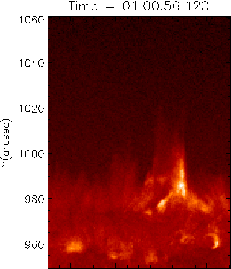
\includegraphics[scale=0.7]{Chapter2/Figs/MS1}
	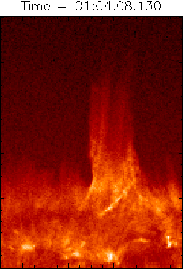
\includegraphics[scale=0.7]{Chapter2/Figs/MS2}
	\caption{The macrospicule examined by \cite{Kayshap2013}. Utilising the $30.4$ nm imager on AIA, the authors closely examine the bright point at the base of the jet.}
\end{figure}


With the limitations of the observations at the time, there was much debate as to whether this was actually the case. 
Following up on the work by \cite{Bohlin1975}, \cite{LaBonte79} utilised the Big Bear Solar Observatory to examine the 'limb surges' in H$\alpha$ and Deuterium 3 (D$_3$).
The authors found that the macrospicules in H$\alpha$ had considerable complexity in their structure, with 'knots, twists and loops' within the confines of the feature.
But in D$_3$, the authors only observe the brightest parts of the macrospicule, usually at the base of the structure apparent in H$\alpha$.
Differently in this case, the authors also observe features on the disk and define three categories: the macrospicules appearing similar to filament eruptions, surge-like macrospicules and a flare brightening type.
Lastly, the paper finds the rate of occurrence of macrospicules to be of the order $~1400$ per solar day. 
This discussion as to the possible links between the two features goes on to this day, more on which later.

The next seminal work on macrospicules was published in \cite{Dere89}, again using an early space station, SpaceLab 2, as the platform for space based observations.
In this case a Gregorian telescope was used to take a series of broadband UV observations at the solar limb.
As a result of this setup the images are a convolution of the intensities from the solar continuum and therefore differentiating between structures is not possible.
This means that only macrospicules' spatial extents could be observed, and specifically those which appeared above the limb, with no study of their onset.
Consequently, this study was statistical in its focus with the aim of being to ascertain the basic spatial properties of the population.

\cite{Dere89} then go on to compare the values obtained in this study to the two previously mentioned.
The papers are generally in agreement, specifically Dere and LaBonte, citing lengths ranging between $3.75$ - $24.75$ Mm and similar widths, although Dere et al. find $0.45$ - $6.75$ Mm and LaBonte $0.45$ - $4.5$. Mm.
The question of velocities is also raised, with values quoted as $20$ - $50$ km s${^{-1}}$ from Dere et al. and $\leq60$ km s${^{-1}}$ from \cite{LaBonte1979}.
These values should possibly be taken with a pinch of salt as the temporal resolution for Dere and Labonte was $20$ or $60$ s and $60$ s respectively, which will greatly influence the measurement of the velocity.
However, Bohlin et al. found more extreme values than all of the other studies.
Some of the lengths they find extend as far as $45$ Mm.
They also find greater widths - $3.75$-$11.25$ Mm - and velocities reaching $150$ km s${^{-1}}$, although again the temporal resolution is poor, $\geq \sim 180$ s.
Although this early work had its limitations, the groundwork was laid here in order to be more precise when more sophisticated missions would be undertaken in the mid $90$s with more focus on detail and less on statistical properties.

With the launch of SoHO in 1996, the community now had continuous viewing of the solar disk, meaning that consistent observations of macrospicules are now possible.
On of the first studies utilising the new instruments was undertaken by \cite{Pike1997} using the Coronal Diagnostic Spectrometer (CDS).
In this case, the instrument scanned from north to south pole, using a mosaic of rastered images, using the He I $58.433$ nm, O V $62.973$ nm and Mg IX $36.806$ lines, corresponding to temperatures of $20,000$, $250,000$ and $1,000,000$ K.
In these observations the macrospicule is apparent at the limb, demonstrating two brightpoints visible in the footpoints either side of the structure, and a fainter column of plasma extending off the limb.
\cite{Pike1997} find that the macrospicule is visible in the He I and O V lines, however not in the higher temperature magnesium line, showing that macrospicules can be found at transition region temperatures, but will not rise to coronal temperatures.
The authors find the macrospicule to be $31$ Mm in height and $13.3$ Mm in width, agreeing with previous values.

The bright roots evident in the O V lines begin to form the 'inverted-Y' shape, typical of the standard jet formation mechanism outlined by \cite{Shibata1992}.
As a result of this, \cite{Pike1997} go on to discuss the nature of the feature and whether it is a macrospicule or X-ray jet.
\cite{Pike1997} conclude that this feature is still classified as a macrospicule, due to the observations in He I and the feature adhering to the properties highlighted in \cite{Bohlin1976}.

Building on the work done by \cite{Pike1997}, \cite{Parenti2002} undertook an extremely detailed case study of a macrospicule observed in CDS.
In this case the observations are still reliant on the macrospicule protruding above the limb, and observed using the full suite of spectra available to the authors.
When discussing these papers, we must consider the rastering method of CDS.
The images are comprised of vertical columns of pixels that are exposed for $30 $ s; the instrument then has a cooldown phase before moving onto the next vertical slit.
This takes approximately $240$ s, which is inappropriate for a feature which on average doesn't have a long lifespan.
Because of this delay, the pixels in the x direction, from one column to the next, are separated by a time of $272$ s.
This means that we cannot consider the spatial structure in the x direction as continuous.
As a result of this the authors use the columns of the image array to identify the temporal resolution of the macrospicule. 

\cite{Parenti2002} find that the macrospicule extends to $26$ Mm and reaches a maximum velocity of $81.6$ km s${^{-1}}$ and an average outflow velocity of $26$ km s${^{-1}}$.
The spectroscopic nature of CDS allows for the calculation of temperature and density.
As the full range of CDS's GIS suite is being used, the density is not strictly a single number and will be dependent on the emission in the various wavelengths.
The density is highest in O IV, $~1.5 \times 10^{10}$ and varies throughout the lines but generally dropping to the order of $10^8$ by the Si IX line.
The temperatures are calculated as ratios between emission lines, \emph{e.g.} O V $62.97$ nm / O IV $55.45$ nm, giving values around $2.0 \times 10^5$ K, which the authors demonstrate is hotter than the surrounding atmosphere at that point, agreeing with previous works by \cite{Habbal1991}. % You don't necessarily need to say so, but be aware that emission ratios are bollocks


As instrumentation improved, the use of spectroscopy resulted in the discovery of the rotational behaviour of a macrospicule as demonstrated in \cite{Kamio2010}.
In this case, the authors are utilising STEREO-A, the Hinode mission and SUMER. 
STEREO was used to observe the feature in $30.4$ for straight-forward imaging, Hinode for dopplergrams and XRT and SUMER for spectroscopic data.

In the lead up to the particular case \cite{Kamio2010} examines, there were multiple coronal jets occurring at the source of the macrospicule over a $9$-hour period.
When the macrospicule erupted, again apparent were two footpoints at the base of the feature in the $30.4$ nm STEREO images, however, in this study there is also a brightening in XRT at the same time. 
This is one of the first concrete examples of the relationship between macrospicules and X-ray jets.
The authors highlight that the two foot-points then go on to form two threads propagating upwards, into the corona, subsequently utilising the SUMER instrument to detect their motion in detail.

% check this section
The properties of this particular example in He II $30.4$ are quoted as $130 \pm 30$ km s${^{-1}}$ for the radial extension of the feature and line-of-sight velocities of the order $-15$ and $-25$ km s${^{-1}}$.
With respect to the X-ray jet behaviour, the velocity is measured at $320 \pm 30$ km s${^{-1}}$ and utilising the LOS velocity in He VIII and Fe XII led \cite{Kamio2010} to conclude that the structure of the macrospicule and X-ray jet.
\cite{Kamio2010} also highlight the regression of the material back to the limb causing an enhancement in He II, a phenomenon they propose is caused by either heating in the upper part of the feature or a result of the density increase caused by the downflow of plasma.

The helical motion of macrospicules is observed in multiple papers.
\cite{Curdt2011} present observations of macrospicules in the transition region; they present two examples of 'explosive events'.
In one case the feature is on the disk and in the second is above the limb.
The discussion at the heart of the paper is differentiating between Rapid Red Extentions/Rapid Blue Extentions (RRE/RBE) pairs and helical motion, due to the fact that they can be misinterpreted in the data.
In this case, the rotational velocity evident in the doppler images demonstrates symmetrical flow of the order $40$ km s${^{-1}}$ for both examples.
Using the slit modes of EIS, the authors rule out the possibility of lateral movement as a result of bidirectional RRE/RBEs, calculating that if this were the case, then the jet would be up to $7.2$ Mm in each doppler component.
This leads to the conclusion that the jet evident at the limb is moving helically, and consequently, that the feature observed on the disk is also a single jet rotating helically.





Numerical sims
Murakowski 2011
